% Author: Jan Schaumann <jschauma@netmeister.org>
% $Id: slides.tex,v 1.13 2005/03/14 21:41:25 jschauma Exp $

% CampusDomain!2011
\special{! TeXDict begin /landplus90{true}store end }

\documentclass[xga]{xdvislides}
\usepackage[landscape]{geometry}
\usepackage{graphics}
\usepackage{graphicx}
\usepackage{colordvi}
\usepackage{multirow}
\usepackage[usenames]{color}
\definecolor{gray}{RGB}{180,180,180}

\begin{document}
\setfontphv

%%% Headers and footers
\lhead{\slidetitle}                               % default:\lhead{\slidetitle}
\chead{CS615 - Aspects of System Administration}% default:\chead{\relax}
\rhead{Slide \thepage}                       % default:\rhead{\sectiontitle}
\lfoot{\Gray{Networking}}% default:\lfoot{\slideauthor}
\cfoot{\relax}                               % default:\cfoot{\relax}
\rfoot{\Gray{\today}}

\vspace*{\fill}
\begin{center}
	\Hugesize
		CS615 - Aspects of System Administration\\ [1em]
		Networking\\ [1em]
	\hspace*{5mm}\blueline\\ [1em]
	\Normalsize
		Department of Computer Science\\
		Stevens Institute of Technology\\
		Jan Schaumann\\
		\verb+jschauma@stevens.edu+\\
		\verb+http://www.cs.stevens.edu/~jschauma/615A/+
\end{center}
\vspace*{\fill}

\subsection{Networking Buzzwords}
\\

\newcommand{\gargantuan}{\fontsize{45}{50}\selectfont}
\gargantuan
\begin{center}
``The network is the computer.'' \\
\small
\vspace*{.5in}
John Gage, Sun Microsystems
\end{center}
\Normalsize

\subsection{Networking Buzzwords}
\\

\gargantuan
\begin{center}
``The network is the network, \\
the computer is the computer - \\
sorry about the confusion.'' \\
\small
\vspace*{.5in}
Joe on Computing
\end{center}
\Normalsize

\subsection{Networking Buzzwords}
\vspace*{\fill}
\begin{center}
	
\includegraphics[scale=0.9]{pics/cloud.eps}
\end{center}
\vspace*{\fill}

\subsection{Networking}
\vspace*{\fill}
\begin{center}
	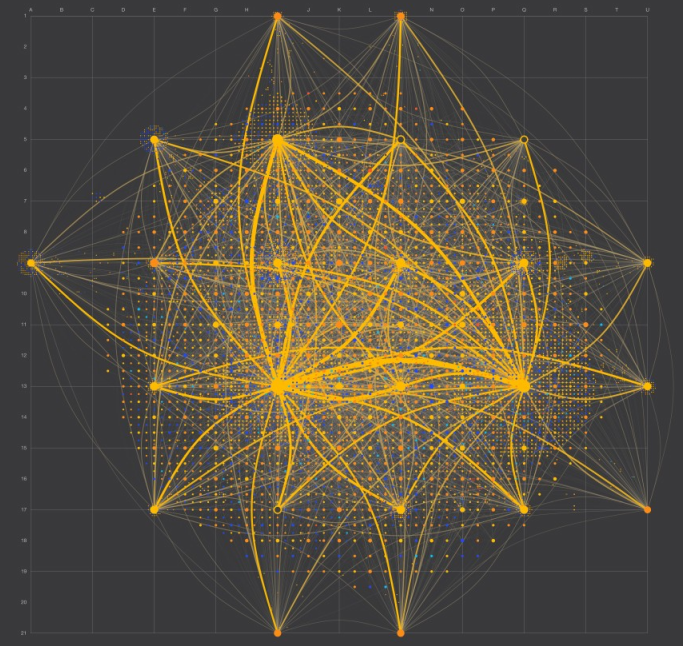
\includegraphics[scale=0.4]{pics/map-of-internet.eps} \\
	\vspace*{\fill}
	\small
	\verb+http://www.peer1.com/map-of-the-internet+ \\
	\verb+http://www.chrisharrison.net/index.php/Visualizations/InternetMap+
	\Normalsize
\end{center}

\subsection{Networking}
\vspace*{\fill}
\begin{center}
	\includegraphics[scale=0.8]{pics/2computers.eps} \\
\end{center}
\vspace*{\fill}

\subsection{Networking}
\vspace*{\fill}
\begin{center}
	\includegraphics[scale=0.8]{pics/3computers.eps} \\
\end{center}
\vspace*{\fill}

\subsection{Networking}
\vspace*{\fill}
\begin{center}
	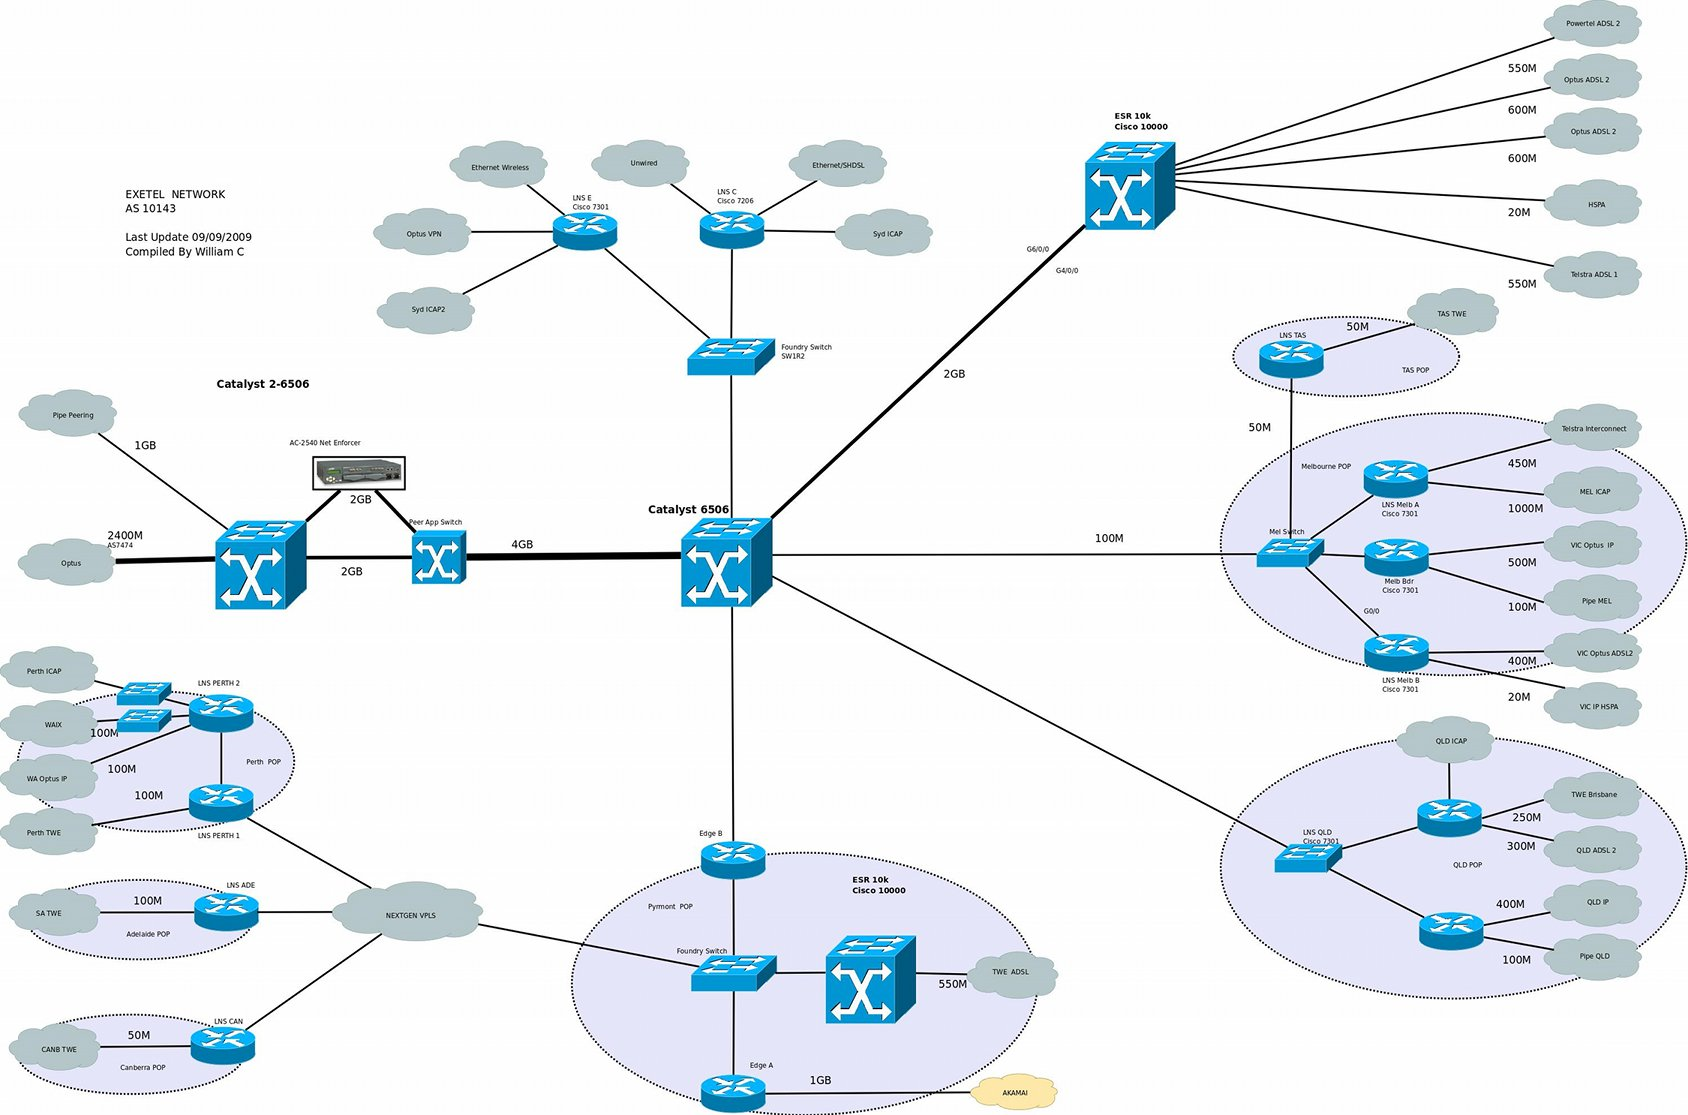
\includegraphics[scale=0.3]{pics/routed.eps} \\
\end{center}
\vspace*{\fill}

\subsection{Networking}
\vspace*{\fill}
\begin{center}
	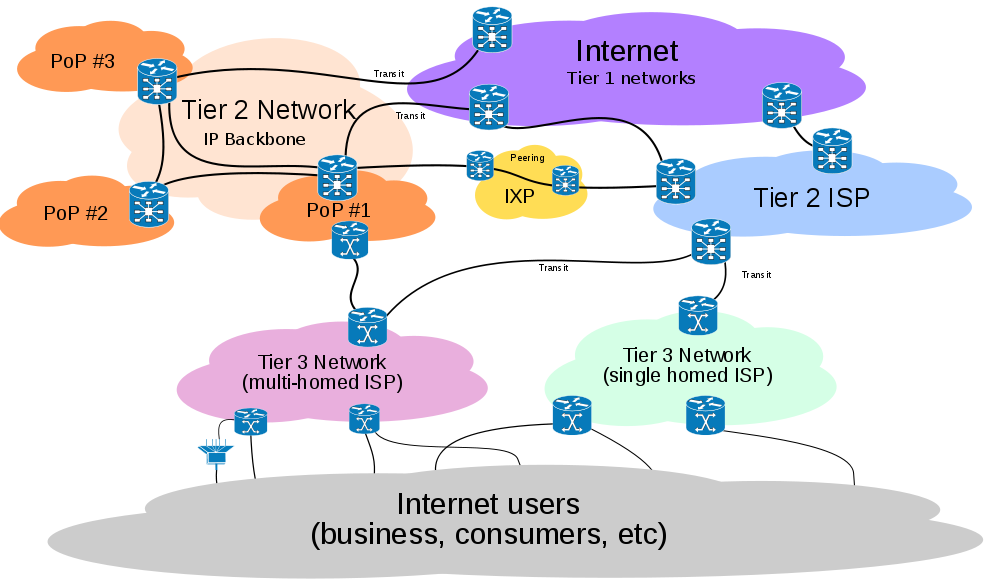
\includegraphics[scale=0.5]{pics/peered-networks.eps} \\
\end{center}
\vspace*{\fill}

\subsection{Networking}
\vspace*{\fill}
\begin{center}
	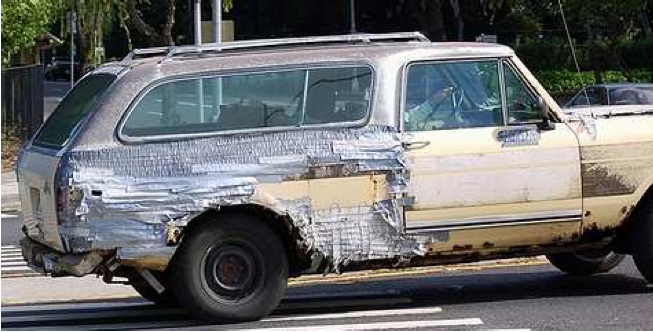
\includegraphics[scale=1.3]{pics/car-duct-tape.eps} \\
\end{center}
\vspace*{\fill}

\subsection{Networking}
\vspace*{\fill}
\begin{center}
	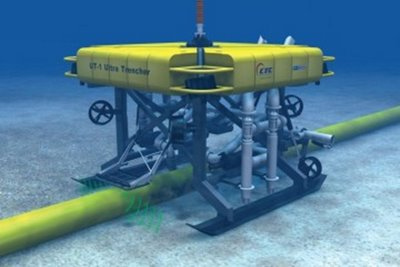
\includegraphics[scale=1.2]{pics/internet-undersea-cable.eps} \\
\end{center}
\vspace*{\fill}


\subsection{Networking}
Stringing cables across the oceans' floors since 1866!
\vspace*{\fill}
\begin{center}
	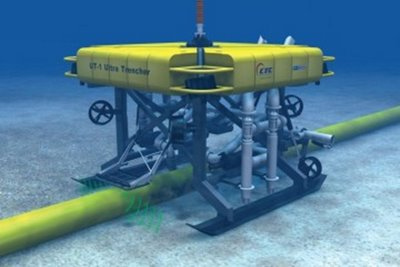
\includegraphics[scale=1.0]{pics/internet-undersea-cable.eps} \\
	\verb+http://www.submarinecablemap.com/+ \\
	\verb+http://is.gd/CjanOu+
\end{center}
\vspace*{\fill}

\subsection{Networking}
\vspace*{\fill}
\begin{center}
	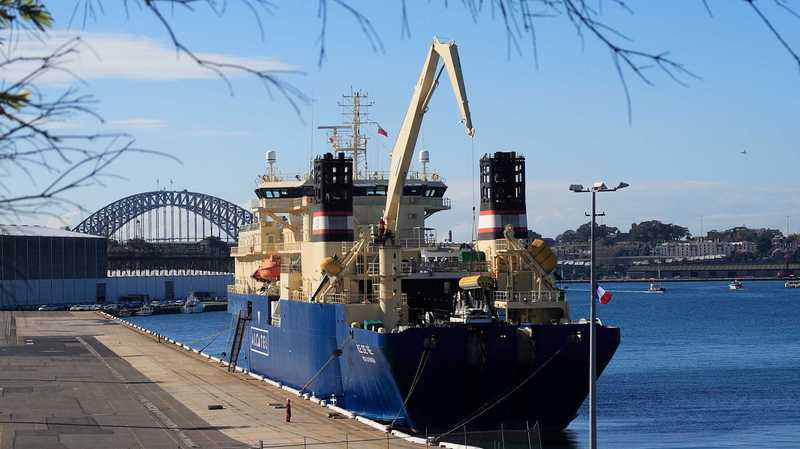
\includegraphics[scale=0.9]{pics/cable-layer.eps} \\
\end{center}
\vspace*{\fill}

\subsection{Networking}
``The Net interprets censorship as damage and routes around it.'' \\

...except when it can't.

\begin{center}
\vspace*{\fill}
	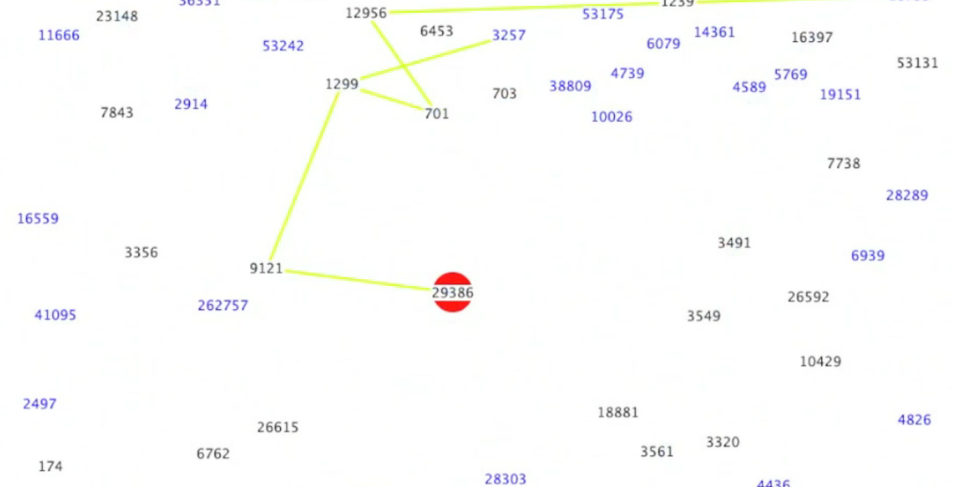
\includegraphics[scale=0.4]{pics/syria-disappears.eps} \\
\vspace*{\fill}

{\tt http://blog.cloudflare.com/how-syria-turned-off-the-internet} \\
{\tt http://player.vimeo.com/video/54630037}
\end{center}

\subsection{Networking}
\begin{center}
\vspace*{\fill}
	
\includegraphics[scale=0.9]{pics/tubes.eps} \\
\vspace*{\fill}
{\tt http://amzn.com/0061994952}
\end{center}





\subsection{A simple example}
\Hugesize
\begin{center}
\begin{verbatim}
$ telnet www.google.com 80

\end{verbatim}
\end{center}
\Normalsize
\vspace*{\fill}

\subsection{A simple example}
\Hugesize
\begin{center}
\begin{verbatim}
$ telnet www.google.com 80
Trying 2607:f8b0:400c:c03::67...
Connected to www.google.com.
Escape character is '^]'.
GET / HTTP/1.0

\end{verbatim}
\end{center}
\Normalsize
\vspace*{\fill}

\subsection{A simple example}
\Hugesize
\begin{center}
\begin{verbatim}
$ telnet www.google.com 80
Trying 2607:f8b0:400c:c03::67...
Connected to www.google.com.
Escape character is '^]'.
GET / HTTP/1.0

HTTP/1.0 200 OK
Date: Mon, 17 Mar 2014 16:15:01 GMT
Content-Type: text/html; charset=ISO-8859-1
Server: gws
[...]
\end{verbatim}
\end{center}
\Normalsize
\vspace*{\fill}


\subsection{A simple example}
What exactly happens?
\\
\begin{itemize}
	\item local host connects to remote host
	\item sends command
	\item receives data
\end{itemize}

\subsection{A simple example}
How exactly do we connect to the remote host?
\\
\begin{itemize}
	\item look up hostname
	\item open connection to IP address
\end{itemize}

\subsection{A simple example}
How exactly do we look up a hostname?
\\
\begin{itemize}
	\item look up various local files
	\item open a connection to a DNS server's IP
	\item ask DNS server to resolve hostname
	\item get back IP
\end{itemize}

\subsection{A simple example}
\\
\Hugesize
\begin{center}
\begin{verbatim}
$ start-fedora
$ ssh fedora@ec2-....
$ sudo yum install -y tcpdump telnet strace
[...]
\end{verbatim}
\end{center}
\Normalsize
\vspace*{\fill}

\subsection{A simple example}
\\
\Hugesize
\begin{center}
\begin{verbatim}
$ strace -f telnet www.google.com 80 2>strace.out
Trying 173.194.73.99...
Connected to www.google.com.
Escape character is '^]'.
GET / HTTP/1.0

[...]
\end{verbatim}
\end{center}
\Normalsize
\vspace*{\fill}

%\subsection{A simple example}
%Let's just look at what files this opens:
%\Hugesize
%\begin{center}
%\begin{verbatim}
%$ strace -f -e trace=open \
%        telnet www.yahoo.com 80 2>strace.out
%Trying 98.139.183.24...
%Connected to any-fp3-real.wa1.b.yahoo.com.
%Escape character is '^]'.
%HEAD / HTTP/1.0
%
%[...]
%\end{verbatim}
%\end{center}
%\Normalsize
%\vspace*{\fill}

\subsection{...open a few files...}
\begin{verbatim}
execve("/usr/bin/telnet", ["telnet", "www.google.com", "80"], [/* 29 vars */]) = 0
[...]
open("/etc/nsswitch.conf", O_RDONLY)    = 3
fstat(3, {st_mode=S_IFREG|0644, st_size=286, ...}) = 0
mmap(NULL, 4096, PROT_READ|PROT_WRITE, MAP_PRIVATE|MAP_ANONYMOUS, -1, 0) = [...]
read(3, "passwd: files ldap\ngroup: files "..., 4096) = 286
[...]
open("/etc/hosts", O_RDONLY|O_CLOEXEC)  = 3
fcntl(3, F_GETFD)                       = 0x1 (flags FD_CLOEXEC)
fstat(3, {st_mode=S_IFREG|0644, st_size=277, ...}) = 0
mmap(NULL, 4096, PROT_READ|PROT_WRITE, MAP_PRIVATE|MAP_ANONYMOUS, -1, 0) = [...]
read(3, "127.0.0.1    localhost\n\n# The fo"..., 4096) = 277
[...]
stat("/etc/resolv.conf", {st_mode=S_IFREG|0644, st_size=205, ...}) = 0
open("/etc/resolv.conf", O_RDONLY)      = 3
fstat(3, {st_mode=S_IFREG|0644, st_size=205, ...}) = 0
read(3, "nameserver 155.246.1.20\nnameserv"..., 4096) = 205
\end{verbatim}

\subsection{... query a DNS server ...}
\begin{verbatim}
[...]
socket(PF_INET, SOCK_DGRAM|SOCK_NONBLOCK, IPPROTO_IP) = 3
connect(3, {sa_family=AF_INET, sin_port=htons(53),
        sin_addr=inet_addr("155.246.1.20")}, 16) = 0
gettimeofday({1330805293, 202924}, NULL) = 0
sendto(3, "\364\333\1\0\0\1\0\0\0\0\0\0\3www\6google\3com\0\0\1\0\1", 32,
        MSG_NOSIGNAL, NULL, 0) = 32
poll([{fd=3, events=POLLIN}], 1, 5000)  = 1 ([{fd=3, revents=POLLIN}])
ioctl(3, FIONREAD, [504])               = 0
recvfrom(3, "\364\333\201\200\0\1\0\6\0\r\0\10\3www\6google\3com\0\0\1\0\1"...,
        1024, 0, {sa_family=AF_INET, sin_port=htons(53),
        sin_addr=inet_addr("155.246.1.20")}, [16]) = 504
close(3)                                = 0
[...]
\end{verbatim}

\subsection{...communicate with the remote host...}
\begin{verbatim}
[...]
write(1, "Trying 173.194.73.104...\n", 25) = 25
close(4294967295)                       = -1 EBADF (Bad file descriptor)
socket(PF_INET, SOCK_STREAM, IPPROTO_IP) = 3
setsockopt(3, SOL_IP, IP_TOS, [16], 4)  = 0
connect(3, {sa_family=AF_INET, sin_port=htons(80),
        sin_addr=inet_addr("173.194.73.104")},16) = 0
[...]
read(0, "GET / HTTP/1.0\n", 8191)       = 15
select(4, [0 3], [3], [3], {0, 0})      = 1 (out [3], left {0, 0})
sendto(3, "GET / HTTP/1.0\r\n", 16, 0, NULL, 0) = 16
[...]
recvfrom(3, "HTTP/1.0 200 OK\r\nDate: Sat, 02 M"..., 8191, 0, NULL, NULL) = 5520
select(4, [0 3], [1], [3], {0, 0})      = 2 (in [3], out [1], left {0, 0})
write(1, "HTTP/1.0 200 OK\nDate: Sat, 02 Ma"..., 5508) = 5508
recvfrom(3, "", 6035, 0, NULL, NULL)    = 0
[...]
\end{verbatim}

% ktrace
%\subsection{A simple example}
%... look up various local files...
%\begin{verbatim}
%[...]
%  5921      1 telnet   CALL  open(0xbba06a65,0,0x1b6)
%  5921      1 telnet   NAMI  "/etc/nsswitch.conf"
%  5921      1 telnet   RET   open 3
%[...]
%  5921      1 telnet   CALL  open(0xbba0474b,0,0x1b6)
%  5921      1 telnet   NAMI  "/etc/hosts"
%  5921      1 telnet   RET   open 3
%[...]
%  5921      1 telnet   CALL  open(0xbba0495b,0,0x1b6)
%  5921      1 telnet   NAMI  "/etc/resolv.conf"
%  5921      1 telnet   RET   open 3
%[...]
%\end{verbatim}
%
%\subsection{A simple example}
%... query a DNS server ...
%\begin{verbatim}
%[...]
%  5921      1 telnet   CALL  socket(2,2,0)
%  5921      1 telnet   RET   socket 3
%  5921      1 telnet   CALL  connect(3,0xbba210f0,0x10)
%  5921      1 telnet   RET   connect 0
%  5921      1 telnet   CALL  sendto(3,0xbfbee0d0,0x1f,0,0,0)
%  5921      1 telnet   GIO   fd 3 wrote 31 bytes
%       "[T\^A\0\0\^A\0\0\0\0\0\0\^Cwww\^Eyahoo\^Ccom\0\0\^\\0\^A"
%[...]
%  5921      1 telnet   CALL  recvfrom(3,0x8077000,0x10000,0,
%                                         0xbfbeda10,0xbfbed9d4)
%  5921      1 telnet   GIO   fd 3 read 139 bytes
%       "[T\M^A\M^@\0\^A\0\^B\0\^A\0\0\^Cwww\^Eyahoo\^Ccom\0\0\^\\0\^A\M-
%  5921      1 telnet   RET   recvfrom 139/0x8b
%  5921      1 telnet   CALL  close(3)
%[...]
%\end{verbatim}
%
%\subsection{A simple example}
%... communicate with remote host ...
%\begin{verbatim}
%  5821      1 telnet   CALL  read(0,0x5222a0,0x400)
%  5821      1 telnet   GIO   fd 0 read 15 bytes
%       "GET / HTTP/1.0\n"
%  5821      1 telnet   RET   read 15/0xf
%  5821      1 telnet   CALL  poll(0x7f7fffffd440,3,0)
%  5821      1 telnet   RET   poll 1
%  5821      1 telnet   CALL  sendto(3,0x521260,0x10,0,0,0)
%  5821      1 telnet   GIO   fd 3 wrote 16 bytes
%       "GET / HTTP/1.0\r\n"
%  5821      1 telnet   RET   sendto 16/0x10
%\end{verbatim}
%\Normalsize
%
%\subsection{A simple example}
%... communicate with remote host ...
%\begin{verbatim}
%  5921      1 telnet   CALL  recvfrom(3,0x8064b80,0x400,0,0,0)
%  5921      1 telnet   GIO   fd 3 read 1024 bytes
%       "HTTP/1.1 200 OK\r
%        Date: Sat, 19 Mar 2011 22:55:56 GMT\r
%        Connection: close\r
%        Content-Type: text/html; charset=utf-8\r
%        <html>
%        <head>
%        <title>Yahoo!</title>
%[...]
%\end{verbatim}
\Normalsize

\subsection{A simple example}
What does this look like on the wire?
\\

\begin{itemize}
	\item determine which nameserver to query
	\item ask who has a route to the nameserver
	\item open socket to well defined port on remote IP
	\item send queries
	\item open socket to requested port on remote IP
\end{itemize}

\subsection{A simple example}
What does this look like on the wire?
\vspace*{1in}
\\
\Hugesize
\begin{center}
\begin{verbatim}
# tcpdump port not 22
\end{verbatim}
\end{center}
\Normalsize
\vspace*{\fill}

\subsection{What does this look like on the wire?}
\begin{verbatim}
$ start-netbsd # custom shell alias
$ ssh <instance-name>
# script commands.out
# ifconfig -a
# route -n get default
# cat /etc/resolv.conf
# tcpdump -w tcpdump.out port not 22 &
# arp -d -a
# telnet www.google.com 80
[...]
# kill %1
# exit
# exit
$ scp <instance-name>:*out ~/tmp/
$ ec2-terminate-instances <instance>
\end{verbatim}

\subsection{A simple example}
Finding the next hop:
\begin{verbatim}
$ tcpdump -n -r tcpdump.out arp
reading from file tcpdump.out, link-type EN10MB (Ethernet)
18:06:59.217533 ARP, Request who-has 10.114.62.1 tell 10.114.63.209, length 28
18:06:59.218187 ARP, Reply 10.114.62.1 is-at fe:ff:ff:ff:ff:ff, length 28
18:07:06.148475 ARP, Request who-has 10.114.63.209 (ff:ff:ff:ff:ff:ff)
                             tell 0.0.0.0, length 28
18:07:06.148499 ARP, Reply 10.114.63.209 is-at 12:31:3d:04:30:23, length 28
18:08:05.820986 ARP, Request who-has 10.114.63.209 (ff:ff:ff:ff:ff:ff)
                             tell 0.0.0.0, length 28
18:08:05.821011 ARP, Reply 10.114.63.209 is-at 12:31:3d:04:30:23, length 28
18:09:18.518859 ARP, Request who-has 10.114.63.209 (ff:ff:ff:ff:ff:ff)
                             tell 0.0.0.0, length 28
18:09:18.518878 ARP, Reply 10.114.63.209 is-at 12:31:3d:04:30:23, length 28
18:10:17.081885 ARP, Request who-has 10.114.63.209 (ff:ff:ff:ff:ff:ff)
                             tell 0.0.0.0, length 28
18:10:17.081903 ARP, Reply 10.114.63.209 is-at 12:31:3d:04:30:23, length 28
\end{verbatim}

\subsection{A simple example}
Performing the DNS query:
\begin{verbatim}
$ tcpdump -t -n -r tcpdump.out udp port 53
reading from file tcpdump.out, link-type EN10MB (Ethernet)
IP 10.202.150.59.65511 > 172.16.0.23.53: 60916+ AAAA? www.google.com. (32)
IP 172.16.0.23.53 > 10.202.150.59.65511: 60916 1/0/0 AAAA 2607:f8b0:400c:c01::93 (60)
IP 10.202.150.59.65510 > 172.16.0.23.53: 1928+ A? www.google.com. (32)
IP 172.16.0.23.53 > 10.202.150.59.65510: 1928 6/0/0 A 173.194.75.105, A
173.194.75.106, A 173.194.75.147, A 173.194.75.99, A 173.194.75.103, A 173.194.75.104 (128)
\end{verbatim}

\subsection{A simple example}
Establishing the connection to the server:
\begin{verbatim}
$ tcpdump -n -r tcpdump.out tcp port 80
IP 10.202.150.59.65531 > 173.194.75.105.80: Flags [S],
        seq 4158935008, win 32768,
        options [mss 1460,nop,wscale 3, ...], length 0
IP 173.194.75.105.80 > 10.202.150.59.65531: Flags [S.],
        seq 933875667, ack 4158935009, win 62920,
        options [mss 1430,nop,nop, ...], length 0
IP 10.202.150.59.65531 > 173.194.75.105.80: Flags [.],
        ack 1, win 4197, length 0
\end{verbatim}

\subsection{A simple example}
Sending the HTTP request:
\begin{verbatim}
IP 10.202.150.59.65531 > 173.194.75.105.80: Flags [P.],
        seq 1:17, ack 1, win 4197, length 16
IP 173.194.75.105.80 > 10.202.150.59.65531: Flags [.],
        ack 17, win 984, length 0
IP 10.202.150.59.65531 > 173.194.75.105.80: Flags [P.],
        seq 17:19, ack 1, win 4197, length 2
IP 173.194.75.105.80 > 10.202.150.59.65531: Flags [.],
        ack 19, win 984, length 0
\end{verbatim}

\subsection{A simple example}
Receiving the HTTP response:
\begin{verbatim}
IP 173.194.75.105.80 > 10.202.150.59.65531: Flags [.],
        seq 1:1431, ack 19, win 984, length 1430
IP 173.194.75.105.80 > 10.202.150.59.65531: Flags [.],
        seq 1431:2861, ack 19, win 984, length 1430
IP 10.202.150.59.65531 > 173.194.75.105.80: Flags [.],
        ack 2861, win 3840, length 0
IP 173.194.75.105.80 > 10.202.150.59.65531: Flags [.],
        seq 2861:4291, ack 19, win 984, length 1430
\end{verbatim}

\subsection{A simple example}
Terminating the connection:
\begin{verbatim}
[...]
IP 10.202.150.59.65531 > 173.194.75.105.80: Flags [.],
        ack 42901, win 3738, length 0
IP 10.202.150.59.65531 > 173.194.75.105.80: Flags [.],
        ack 42901, win 4122, length 0
IP 173.194.75.105.80 > 10.202.150.59.65531: Flags [.],
        seq 42901:44331, ack 19, win 984, length 1430
IP 173.194.75.105.80 > 10.202.150.59.65531: Flags [FP.],
        seq 44331:44839, ack 19, win 984, length 508
IP 10.202.150.59.65531 > 173.194.75.105.80: Flags [.],
        ack 44840, win 4134, length 0
IP 10.202.150.59.65531 > 173.194.75.105.80: Flags [F.],
        seq 19, ack 44840, win 4197, length 0
IP 173.194.75.105.80 > 10.202.150.59.65531: Flags [.],
        ack 20, win 984, length 0
\end{verbatim}

\subsection{Notables from this simple example}
``Simple'' is, as usual, relative.
\\

\begin{itemize}
	\item host configuration assumed
\end{itemize}

\subsection{Notables from this simple example}
``Simple'' is, as usual, relative.
\\

\begin{itemize}
	\item host configuration assumed
	\item network architecture (internal or across the internet) not
			relevant (here)
\end{itemize}

\subsection{Notables from this simple example}
``Simple'' is, as usual, relative.
\\

\begin{itemize}
	\item host configuration assumed
	\item network architecture (internal or across the internet) not
			relevant (here)
	\item even simple examples cross multiple layers and protocols
			(HTTP, DNS; TCP, UDP, ARP)
\end{itemize}

\subsection{Notables from this simple example}
``Simple'' is, as usual, relative.
\\

\begin{itemize}
	\item host configuration assumed
	\item network architecture (internal or across the internet) not
			relevant (here)
	\item even simple examples cross multiple layers and protocols
			(HTTP, DNS; TCP, UDP, ARP)
	\item we haven't even scratched the surface
\end{itemize}

\subsection{TCP/IP Basics: Protocol Layers}
\begin{center}
	\begin{tabular}{|cl|l|}
	\hline
	& {\bf Layer} & {\bf Function} \\
	\hline
	4. & Application Layer & End-User application programs \\
	3. & Transport Layer & Delivery of data to applications \\
	2. & Network Layer & Basic communication, addressing, and routing \\
	\multirow{2}{*}{1.} & Link Layer & Network Hardware and device drivers \\
	& Physical Layer & Cable or physical medium \\
	\hline
	\end{tabular}
\end{center}
\addvspace{.5in}
Examples of protocols for each layer:
\begin{itemize}
	\item Simple Mail Transfer Protocol (RFC 821) \\
		Hypertext Transfer Protocol (RFC 2616)
	\item Transmission Control Protocol (RFC 793, tcp(4)) \\
		User Datagram Protocol (RFC 768; udp(4))
	\item Internet Protocol (RFC 791; ip(4)) \\
		Internet Control Message Protocol (RFC 792; icmp(4))
	\item Address Resolution Protocol (RFC 826; arp(4))
\end{itemize}

\subsection{TCP/IP Basics: Protocol Layers (OSI Model)}
\vspace*{\fill}
\begin{center}
	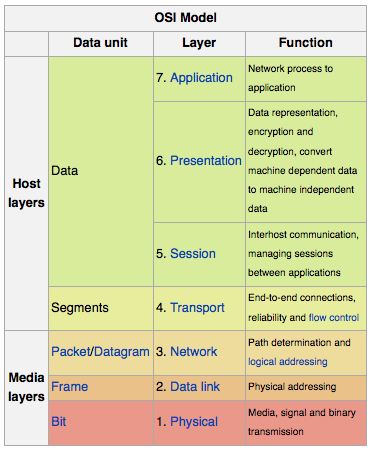
\includegraphics[scale=0.7]{pics/osi.eps}
\end{center}
\vspace*{\fill}

\subsection{TCP/IP Basics: ARP}
\begin{center}
Ethernet Address Resolution Protocol \\
-- or -- \\
Converting Network Protocol Addresses to 48-bit Ethernet Address for Transmission on Ethernet Hardware
\end{center}

\begin{verbatim}
$ arp -a
logger.srcit.stevens-tech.edu (155.246.89.81) at 00:07:e9:09:c8:94 [ether] on eth0
vader.srcit.stevens-tech.edu (155.246.89.5) at 00:23:8b:a9:dd:60 [ether] on eth0
tarantula.phy.stevens-tech.edu (155.246.89.41) at 00:50:45:5f:1c:d4 [ether] on eth0
nirvana.phy.stevens-tech.edu (155.246.89.33) at 00:1e:68:0f:99:a2 [ether] on eth0
Vlan16.cc.stevens-tech.edu (155.246.89.1) at 00:09:44:d1:64:00 [ether] on eth0
cinema.srcit.stevens-tech.edu (155.246.89.67) at 00:25:90:1e:05:51 [ether] on eth0
\end{verbatim}

\subsection{TCP/IP Basics: ARP}
\vspace*{\fill}
\begin{center}
	\includegraphics[scale=0.8]{pics/3computers-arp.eps}
\end{center}
\vspace*{\fill}


\subsection{TCP/IP Basics: ARP}
\begin{center}
Ethernet Address Resolution Protocol \\
-- or -- \\
Converting Network Protocol Addresses to 48-bit Ethernet Address for Transmission on Ethernet Hardware
\end{center}
\vspace{.2in}

\begin{verbatim}
18:06:59.217533 ARP, Request who-has 10.114.62.1 tell 10.114.63.209, length 28
18:06:59.218187 ARP, Reply 10.114.62.1 is-at fe:ff:ff:ff:ff:ff, length 28
18:07:06.148475 ARP, Request who-has 10.114.63.209 (ff:ff:ff:ff:ff:ff)
                             tell 0.0.0.0, length 28
18:07:06.148499 ARP, Reply 10.114.63.209 is-at 12:31:3d:04:30:23, length 28
18:08:05.820986 ARP, Request who-has 10.114.63.209 (ff:ff:ff:ff:ff:ff)
                             tell 0.0.0.0, length 28
18:08:05.821011 ARP, Reply 10.114.63.209 is-at 12:31:3d:04:30:23, length 28
18:09:18.518859 ARP, Request who-has 10.114.63.209 (ff:ff:ff:ff:ff:ff)
                             tell 0.0.0.0, length 28
18:09:18.518878 ARP, Reply 10.114.63.209 is-at 12:31:3d:04:30:23, length 28
\end{verbatim}

\subsection{TCP/IP Basics: ND}
\begin{center}
Neighbor Discovery Protocol
\end{center}
\vspace{.2in}

\begin{verbatim}
$ ndp -n -a
Neighbor                            Linklayer Address  Netif Expire      S Flags
2001:470:30:84:e276:63ff:fe72:3900  e0:76:63:72:39:00  xennet0 permanent R
fe80::21b:21ff:fe45:bf54%xennet0    00:1b:21:45:bf:54  xennet0 21m52s    S R
fe80::21b:21ff:fe7a:7269%xennet0    00:1b:21:7a:72:69  xennet0 23h59m59s S R
fe80::e276:63ff:fe72:3900%xennet0   e0:76:63:72:39:00  xennet0 permanent R
fe80::1%lo0                          (incomplete)      lo0     permanent R
$
\end{verbatim}

\subsection{TCP/IP Basics: ND}
\begin{center}
Neighbor Discovery Protocol
\end{center}
\vspace{.2in}
\begin{verbatim}
22:35:47.947624 IP6 fe80::21b:21ff:fe7a:7269 > ff02::1:ff62:3400: ICMP6,
        neighbor solicitation, who has 2001:470:30:84:e276:63ff:fe62:3400, length 32
22:35:50.950101 IP6 2001:470:30:84:e276:63ff:fe72:3900 > ff02::1:ff7a:7269: ICMP6,
        neighbor solicitation, who has fe80::21b:21ff:fe7a:7269, length 32
22:35:50.950690 IP6 fe80::21b:21ff:fe7a:7269 > 2001:470:30:84:e276:63ff:fe72:3900:
        ICMP6, neighbor advertisement, tgt is fe80::21b:21ff:fe7a:7269, length 32
\end{verbatim}

\subsection{TCP/IP Basics: ICMP}
\begin{center}
Internet Control Message Protocol
\end{center}
\vspace{.2in}

\begin{verbatim}
$ ping -c 3 www.yahoo.com
PING any-fp.wa1.b.yahoo.com (67.195.160.76): 56 data bytes
64 bytes from 67.195.160.76: icmp_seq=0 ttl=53 time=30.888 ms
64 bytes from 67.195.160.76: icmp_seq=1 ttl=53 time=23.193 ms
64 bytes from 67.195.160.76: icmp_seq=2 ttl=53 time=25.433 ms

----any-fp.wa1.b.yahoo.com PING Statistics----
3 packets transmitted, 3 packets received, 0.0% packet loss
round-trip min/avg/max/stddev = 23.193/26.505/30.888/3.958 ms
$
\end{verbatim}

\subsection{TCP/IP Basics: ICMP: Ping}
\vspace*{\fill}
\begin{center}
	\includegraphics[scale=0.8]{pics/3computers-ping.eps}
\end{center}
\vspace*{\fill}


\subsection{TCP/IP Basics: ICMP}
\begin{center}
Internet Control Message Protocol
\end{center}
\vspace{.2in}

\begin{verbatim}
13:23:03.081954 IP 166.84.7.99 > 67.195.160.76: icmp 64: echo request seq 23
13:23:03.092153 IP 67.195.160.76 > 166.84.7.99: icmp 64: echo reply seq 23
13:23:04.081865 IP 166.84.7.99 > 67.195.160.76: icmp 64: echo request seq 24
13:23:04.090909 IP 67.195.160.76 > 166.84.7.99: icmp 64: echo reply seq 24
13:23:05.071735 IP 166.84.7.99 > 67.195.160.76: icmp 64: echo request seq 25
13:23:05.081368 IP 67.195.160.76 > 166.84.7.99: icmp 64: echo reply seq 25
\end{verbatim}


\subsection{TCP/IP Basics: ICMP6}
\begin{center}
Internet Control Message Protocol for IPv6
\end{center}
\vspace{.2in}

\begin{verbatim}
$ ping6 -c 3 www.netbsd.org
PING6(56=40+8+8 bytes) 2001:470:30:84:204:d7b0:0:1 -->
                       2001:4f8:3:7:2e0:81ff:fe52:9a6b
16 bytes from 2001:4f8:3:7:2e0:81ff:fe52:9a6b, icmp_seq=0 hlim=57 time=74.316 ms
16 bytes from 2001:4f8:3:7:2e0:81ff:fe52:9a6b, icmp_seq=1 hlim=57 time=71.260 ms
16 bytes from 2001:4f8:3:7:2e0:81ff:fe52:9a6b, icmp_seq=2 hlim=57 time=71.321 ms

--- www.netbsd.org ping6 statistics ---
3 packets transmitted, 3 packets received, 0.0% packet loss
round-trip min/avg/max/std-dev = 71.260/72.299/74.316/1.747 ms
\end{verbatim}

\subsection{TCP/IP Basics: ICMP6}
\begin{center}
Internet Control Message Protocol for IPv6
\end{center}
\vspace{.2in}

\begin{verbatim}
12:46:58.524431 IP6 2001:470:30:84:204:d7b0:0:1 >
   2001:4f8:3:7:2e0:81ff:fe52:9a6b: ICMP6, echo reque st, seq 0, length 16
12:46:58.598621 IP6 2001:4f8:3:7:2e0:81ff:fe52:9a6b >
   2001:470:30:84:204:d7b0:0:1: ICMP6, echo reply , seq 0, length 16
12:46:59.532864 IP6 2001:470:30:84:204:d7b0:0:1 >
   2001:4f8:3:7:2e0:81ff:fe52:9a6b: ICMP6, echo request, seq 1, length 16
12:46:59.604011 IP6 2001:4f8:3:7:2e0:81ff:fe52:9a6b >
   2001:470:30:84:204:d7b0:0:1: ICMP6, echo reply , seq 1, length 16
12:47:00.532817 IP6 2001:470:30:84:204:d7b0:0:1 >
   2001:4f8:3:7:2e0:81ff:fe52:9a6b: ICMP6, echo reque st, seq 2, length 16
12:47:00.604016 IP6 2001:4f8:3:7:2e0:81ff:fe52:9a6b >
   2001:470:30:84:204:d7b0:0:1: ICMP6, echo reply , seq 2, length 16
\end{verbatim}

\subsection{TCP/IP Basics: ICMP: Traceroute}
\vspace*{\fill}
\begin{center}
	\includegraphics[scale=0.8]{pics/traceroute1.eps}
\end{center}
\vspace*{\fill}

\subsection{TCP/IP Basics: ICMP: Traceroute}
\vspace*{\fill}
\begin{center}
	\includegraphics[scale=0.8]{pics/traceroute2.eps}
\end{center}
\vspace*{\fill}

\subsection{TCP/IP Basics: ICMP: Traceroute}
\vspace*{\fill}
\begin{center}
	\includegraphics[scale=0.8]{pics/traceroute3.eps}
\end{center}
\vspace*{\fill}

\subsection{TCP/IP Basics: ICMP: Traceroute}
\vspace*{\fill}
\begin{center}
	\includegraphics[scale=0.8]{pics/traceroute4.eps}
\end{center}
\vspace*{\fill}



\subsection{TCP/IP Basics: ICMP}
\begin{center}
Internet Control Message Protocol
\end{center}
\vspace{.2in}

\begin{verbatim}
$ traceroute www.netbsd.org
traceroute to www.netbsd.org (204.152.190.12), 64 hops max, 40 byte packets
 1  eth2-3a.core1.nav.nyc.access.net (166.84.0.1)  0.256 ms  0.165 ms 0.181 ms
 2  l3v1.nyc.access.net (166.84.66.14)  1.570 ms  1.556 ms  1.437 ms
 3  gige-g3-3.core1.nyc4.he.net (209.51.171.25)  4.963 ms  2.422 ms  1.457 ms
 4  10gigabitethernet2-3.core1.ash1.he.net (72.52.92.86)  8.423 ms  8.769 ms  7.683 ms
 5  10gigabitethernet1-2.core1.atl1.he.net (184.105.213.110)  21.898 ms 19.647 ms  19.838 ms
 6  isc.gige-g2-1.core1.atl1.he.net (216.66.0.50)  77.465 ms  77.921 ms 80.519 ms
 7  iana.r1.atl1.isc.org (199.6.12.1)  77.302 ms  78.230 ms  81.782 ms
 8  int-0-5-0-1.r1.pao1.isc.org (149.20.65.37)  81.860 ms  83.780 ms 84.160 ms
 9  int-0-0-1-0.r1.sql1.isc.org (149.20.65.10)  81.543 ms  80.193 ms 84.434 ms
10  www.netbsd.org (204.152.190.12)  81.986 ms  81.008 ms  82.604 ms
$
\end{verbatim}

\subsection{TCP/IP Basics: ICMP}
\begin{center}
Internet Control Message Protocol
\end{center}

\begin{verbatim}
14:36:30.023140 IP 166.84.7.99.45320 > 204.152.190.12.33435: UDP, length 12
14:36:30.023364 IP 166.84.0.1 > 166.84.7.99: ICMP time exceeded in-transit
14:36:30.024440 IP 166.84.7.99.45320 > 204.152.190.12.33438: UDP, length 12
14:36:30.025984 IP 166.84.66.14 > 166.84.7.99: ICMP time exceeded in-transit
14:36:30.029685 IP 166.84.7.99.45320 > 204.152.190.12.33441: UDP, length 12
14:36:30.034620 IP 209.51.171.25 > 166.84.7.99: ICMP time exceeded in-transit
14:36:30.039199 IP 166.84.7.99.45320 > 204.152.190.12.33444: UDP, length 12
14:36:30.047596 IP 72.52.92.86 > 166.84.7.99: ICMP time exceeded in-transit
[...]
14:36:31.572154 IP 149.20.65.37 > 166.84.7.99: ICMP time exceeded in-transit
14:36:31.820942 IP 166.84.7.99.45320 > 204.152.190.12.33460: UDP, length 12
14:36:31.901093 IP 149.20.65.10 > 166.84.7.99: ICMP time exceeded in-transit
14:36:31.985765 IP 166.84.7.99.45320 > 204.152.190.12.33462: UDP, length 12
14:36:32.067707 IP 204.152.190.12 > 166.84.7.99: ICMP 204.152.190.12
                         udp port 33462 unreachable, len gth 36
\end{verbatim}


\subsection{TCP/IP Basics: ICMP6}
\begin{center}
Internet Control Message Protocol for IPv6
\end{center}
\vspace{.2in}

\begin{verbatim}
$ traceroute6 www.netbsd.org
traceroute6 to www.netbsd.org (2001:4f8:3:7:2e0:81ff:fe52:9a6b) from
    2001:470:30:84:204:d7b0:0:1, 64 hops max, 12 byte packets
 1  router.vc.panix.com  0.271 ms  0.282 ms  0.155 ms
 2  2001:470:30::a654:420e  5.459 ms  1.251 ms  1.073 ms
 3  gige-g3-3.core1.nyc4.he.net  1.288 ms  2.001 ms  10.176 ms
 4  10gigabitethernet8-3.core1.chi1.he.net  26.603 ms  20.532 ms  25.029 ms
 5  2001:470:1:34::2  72.033 ms  72.377 ms  72.686 ms
 6  iana.r1.ord1.isc.org  76.288 ms  72.773 ms  71.481 ms
 7  int-0-0-1-8.r1.pao1.isc.org  73.027 ms  76.489 ms  77.507 ms
 8  int-0-0-1-0.r2.sql1.isc.org  73.555 ms  75.367 ms  74.769 ms
 9  www.NetBSD.org  72.036 ms  72.522 ms  71.39 ms
$
\end{verbatim}

\subsection{TCP/IP Basics: ICMP}
\vfill
\verb+traceroute -m 254 -q1 obiwan.scrye.net+
\vfill

\subsection{TCP/IP Basics: ICMP6}
\begin{center}
Internet Control Message Protocol for IPv6
\end{center}

\begin{verbatim}
12:47:26.860045 IP6 2001:470:30:84:204:d7b0:0:1.51749 >
                    2001:4f8:3:7:2e0:81ff:fe52:9a6b.33435: UDP, length 12
12:47:26.860265 IP6 2001:470:30:84::3 > 2001:470:30:84:204:d7b0:0:1:
                    ICMP6, time exceeded in-transit [|icmp6]
12:47:26.860907 IP6 2001:470:30:84:204:d7b0:0:1.51749 >
                    2001:4f8:3:7:2e0:81ff:fe52:9a6b.33436: UDP, length 12
[...]
12:47:29.759506 IP6 2001:470:30:84:204:d7b0:0:1.51749 >
                    2001:4f8:3:7:2e0:81ff:fe52:9a6b.33461: UDP, length 12
12:47:29.830787 IP6 2001:4f8:3:7:2e0:81ff:fe52:9a6b >
                    2001:470:30:84:204:d7b0:0:1: ICMP6,
                         destination unreachable[|icmp6]
\end{verbatim}

\subsection{TCP/IP Basics: TCP}
\begin{center}
Transmission Control Protocol
\end{center}
\vspace{.2in}
\begin{verbatim}
$ telnet www.google.com 80
Trying 173.194.73.99...
Connected to www.google.com.
Escape character is '^]'.
GET / HTTP/1.0

\end{verbatim}

\subsection{TCP/IP Basics: TCP}
\begin{center}
Transmission Control Protocol
\end{center}
\vspace{.2in}
\begin{verbatim}
14:51:33.582076 IP 166.84.7.99.58356 > 67.195.160.76.80: S
      2267539609:2267539609(0) win 32768
      <mss 1460,nop,wscale 3,sackOK,nop,nop,nop,nop,timestamp 10>
14:51:33.590748 IP 67.195.160.76.80 > 166.84.7.99.58356: S
      3229501874:3229501874(0) ack 2267539610 win 5792
      <mss 1440,sackOK,timestamp 1241180702 1,nop,wscale 8>
14:51:33.590766 IP 166.84.7.99.58356 > 67.195.160.76.80: .
      ack 1 win 4197 <nop,nop,timestamp 1 1241180702>
14:51:37.732720 IP 166.84.7.99.58356 > 67.195.160.76.80: P
      1:17(16) ack 1 win 4197 <nop,nop,timestamp 9 1241180702>
14:51:37.741763 IP 67.195.160.76.80 > 166.84.7.99.58356: .
      ack 17 win 23 <nop,nop,timestamp 12411848 53 9>
\end{verbatim}

\subsection{TCP/IP Basics: TCP}
\begin{center}
Transmission Control Protocol over IPv6
\end{center}
\vspace{.2in}
\begin{verbatim}
$ telnet www.netbsd.org 80
Trying 2001:4f8:3:7:2e0:81ff:fe52:9a6b...
Connected to www.netbsd.org.
Escape character is '^]'.
GET / HTTP/1.0


\end{verbatim}

\subsection{TCP/IP Basics: TCP}
\begin{center}
Transmission Control Protocol IPv6
\end{center}
\vspace{.2in}
\begin{verbatim}
14:58:11.128436 IP6 2001:470:30:84:204:d7b0:0:1.58334 >
      2001:4f8:3:7:2e0:81ff:fe52:9a6b.80: S 3232473102:3232473102(0)
      win 32768 <mss 1440,nop,wscale3,sackOK,nop,nop,nop,nop,timestamp 1[|tcp]>
14:58:11.200293 IP6 2001:4f8:3:7:2e0:81ff:fe52:9a6b.80 >
      2001:470:30:84:204:d7b0:0:1.58334: S 4139493123:4139493123(0)
      ack 3232473103 win 32768
14:58:11.200337 IP6 2001:470:30:84:204:d7b0:0:1.58334 >
      2001:4f8:3:7:2e0:81ff:fe52:9a6b.80: . ack 1 win 4140
14:58:14.322701 IP6 2001:470:30:84:204:d7b0:0:1.58334 >
      2001:4f8:3:7:2e0:81ff:fe52:9a6b.80: P 1:17(16) ack 1 win 4140
14:58:14.589416 IP6 2001:4f8:3:7:2e0:81ff:fe52:9a6b.80 >
      2001:470:30:84:204:d7b0:0:1.58334: . ack 17 win 33120
14:58:14.752420 IP6 2001:470:30:84:204:d7b0:0:1.58334 >
\end{verbatim}


\subsection{TCP/IP Basics: UDP}
\begin{center}
User Datagram Protocol
\end{center}
\vspace{.2in}
\begin{verbatim}
$ nslookup www.yahoo.com
Server:		155.246.1.20
Address:	155.246.1.20#53

Non-authoritative answer:
www.yahoo.com        canonical name = fp3.wg1.b.yahoo.com.
fp3.wg1.b.yahoo.com       canonical name = any-fp3-lfb.wa1.b.yahoo.com.
any-fp3-lfb.wa1.b.yahoo.com        canonical name = any-fp3-real.wa1.b.yahoo.com.
Name:	any-fp3-real.wa1.b.yahoo.com
Address: 98.139.183.24

$
\end{verbatim}

\subsection{TCP/IP Basics: UDP}
\begin{center}
User Datagram Protocol
\end{center}
\vspace{.2in}
\begin{verbatim}
15:06:04.760444 IP (tos 0x0, ttl 64, id 0, offset 0, flags [none],
    proto UDP (17), length 59) panix.netmeister.org.49164 >
        cache2.ns.access.net.domain: 28557+ A? www.yahoo.com. (31)

15:06:05.210569 IP (tos 0x0, ttl 63, id 1862, offset 0, flags [none],
    proto UDP (17), length 207) cache2.ns.access.net.domain >
        panix.netmeister.org.49164: 28557 4/2/2
            www.yahoo.com. CNAME fp3.wg1.b.yahoo.com.[|domain]
\end{verbatim}

\subsection{TCP/IP Basics: UDP}
\begin{center}
User Datagram Protocol over IPv6
\end{center}
\vspace{.2in}
\begin{verbatim}
$ dig -6 @2001:470:20::2 www.yahoo.com

;; ANSWER SECTION:
www.yahoo.com.          300     IN      CNAME   fp3.wg1.b.yahoo.com.
fp3.wg1.b.yahoo.com.    60      IN      CNAME   any-fp3-lfb.wa1.b.yahoo.com.
any-fp3-lfb.wa1.b.yahoo.com. 300 IN     CNAME   any-fp3-real.wa1.b.yahoo.com.
any-fp3-real.wa1.b.yahoo.com. 60 IN     A       98.139.183.24

;; Query time: 51 msec
;; SERVER: 2001:470:20::2#53(2001:470:20::2)
;; WHEN: Sat Mar  3 22:49:44 2012
;; MSG SIZE  rcvd: 128

\end{verbatim}

\subsection{TCP/IP Basics: UDP}
\begin{center}
User Datagram Protocol over IPv6
\end{center}
\vspace{.2in}
\begin{verbatim}
15:24:20.731990 IP6 (hlim 64, next-header: UDP (17), length: 39)
       2001:470:30:84:204:d7b0:0:1.65037 > 2001:470:20::2.53:
       [udp sum ok] 18545+ A? www.yahoo.com. (31)

15:24:20.976796 IP6 (hlim 61, next-header: UDP (17), length: 119)
       2001:470:20::2.53 > 2001:470:30:84:204:d7b0:0:1.65037:
       18545 4/0/0 www.yahoo.com.[|domain]

\end{verbatim}



\subsection{TCP/IP Basics: Putting it all together}
\vspace*{\fill}
\begin{center}
	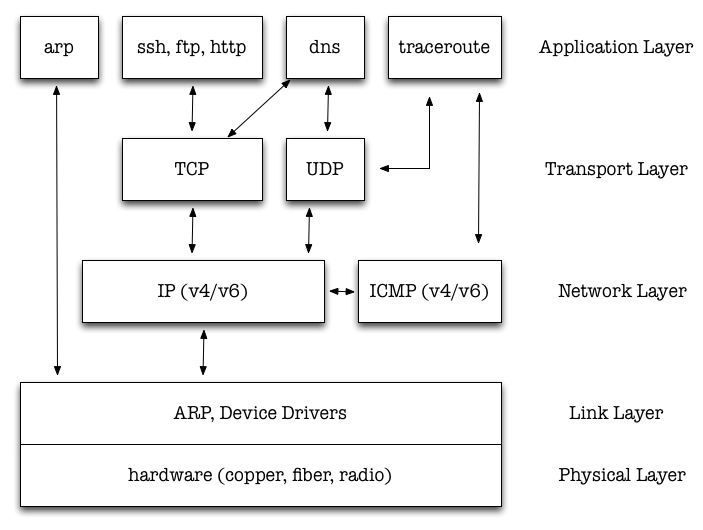
\includegraphics[scale=0.6]{pics/tcpip-stack.eps}
\end{center}
\vspace*{\fill}


\newpage
\vspace*{\fill}
\begin{center}
    \Hugesize
        Hooray! \\ [1em]
    \hspace*{5mm}
    \blueline\\
    \hspace*{5mm}\\
        5 Minute Break
\end{center}
\vspace*{\fill}

% \subsection{IPv4 Basics}
% \vspace{.5in}
% \Hugesize
% \begin{center}
% \begin{verbatim}
%       10011011111101100101100100010110
% \end{verbatim}
% \vspace{.5in}
% IPv4 addresses are 32-bit numbers.
% \end{center}
% \Normalsize
%
% \subsection{IPv4 Basics}
% \vspace{.5in}
% \Hugesize
% \begin{center}
% \begin{verbatim}
%      1001101111110110  0101100100010110
% \end{verbatim}
% \vspace{.5in}
% IPv4 addresses are divided into a {\em network part} and a {\em host part}.
% \end{center}
% \Normalsize
%
% \subsection{IPv4 Basics}
% \vspace{.5in}
% \Hugesize
% \begin{center}
% \begin{verbatim}
%      10  01101111110110  0101100100010110
% \end{verbatim}
% \vspace{.5in}
% There are three different {\em classes} of IPv4 networks.
% \end{center}
% \Normalsize
%
% \subsection{IPv4 Basics}
% \vspace{.5in}
% \Hugesize
% \begin{center}
% \begin{verbatim}
%      10011011  11110110  01011001  00010110
% \end{verbatim}
% \vspace{.5in}
% Each IPv4 address consists of four octets.
% \end{center}
% \Normalsize
%
% \subsection{IPv4 Basics}
% \vspace{.5in}
% \Hugesize
% \begin{center}
% \begin{verbatim}
%     10011011  11110110  01011001  00010110
%
%       155   .   246   .    89   .    22
% \end{verbatim}
% \vspace{.5in}
% Each IPv4 address consists of four octets.
% \end{center}
% \Normalsize
%
% \subsection{Subnets}
% \vspace{.5in}
% \Hugesize
% \begin{center}
% \begin{verbatim}
%     10011011  11110110  01011001  00010110
%
%     11111111  11111111  00000000  00000000
% \end{verbatim}
% \vspace{.5in}
% A {\em netmask} splits the IPv4 address into {\em network} and {\em host}
% parts.
% \end{center}
% \Normalsize
%
% \subsection{Subnets}
% \vspace{.5in}
% \Hugesize
% \begin{center}
% \begin{verbatim}
%     10011011  11110110  01011001  00010110
%
%     11111111  11111111  11111111  00000000
% \end{verbatim}
% \vspace{.5in}
% A {\em netmask} splits the IPv4 address into {\em network} and {\em host}
% parts.
% \end{center}
% \Normalsize
%
% \subsection{Subnets}
% \begin{verbatim}
% $ ipcalc -n 155.246.89.22/16
% Address:   155.246.89.22        10011011.11110110. 01011001.00010110
% Netmask:   255.255.0.0 = 16     11111111.11111111. 00000000.00000000
% Wildcard:  0.0.255.255          00000000.00000000. 11111111.11111111
% =>
% Network:   155.246.0.0/16       10011011.11110110. 00000000.00000000
% HostMin:   155.246.0.1          10011011.11110110. 00000000.00000001
% HostMax:   155.246.255.254      10011011.11110110. 11111111.11111110
% Broadcast: 155.246.255.255      10011011.11110110. 11111111.11111111
% Hosts/Net: 65534                 Class B
% \end{verbatim}
% \vspace{.5in}
% Try also: \verb+sipcalc -a 155.246.89.22/16+
%
% \subsection{Subnets}
% \begin{verbatim}
% $ ipcalc -n 155.246.89.22/24
% Address:   155.246.89.22        10011011.11110110.01011001. 00010110
% Netmask:   255.255.255.0 = 24   11111111.11111111.11111111. 00000000
% Wildcard:  0.0.0.255            00000000.00000000.00000000. 11111111
% =>
% Network:   155.246.89.0/24      10011011.11110110.01011001. 00000000
% HostMin:   155.246.89.1         10011011.11110110.01011001. 00000001
% HostMax:   155.246.89.254       10011011.11110110.01011001. 11111110
% Broadcast: 155.246.89.255       10011011.11110110.01011001. 11111111
% Hosts/Net: 254                   Class B
% \end{verbatim}
% \vspace{.5in}
% Try also: \verb+sipcalc -a 155.246.89.22/16+
%
% \subsection{CIDR cheat sheet}
% A.B.C.D/N
% \begin{itemize}
% 	\item $N$ = bits describing network portion of address
% 	\item $M=32-N$ = bits in host portion of address
% 	\item $2^M$ = number of addresses on this subnet
% 	\item $2^M - 2$ = number of possible hosts
% 		\begin{itemize}
% 			\item first address on subnet = network address
% 			\item last address on subnet = broadcast address
% 		\end{itemize}
% 	\item subnet division need not occur on dotted boundary only
% 		\begin{itemize}
% 			\item for example, you can divide 155.246.89.0/24
% 				into four /26 networks
% 			\item networks starting at .0, .64, .128, .192
% 		\end{itemize}
% \end{itemize}
% \addvspace{.5in}
% Which of the following is not a valid netmask? \\
% \verb+255.255.253.0, 255.255.250.0, 255.255.240.0+
%
% \subsection{Mommy, where do IP addresses come from?}
% \Huge
% \vfill
% \begin{center}
% The Internet Assigned Numbers Authority (IANA) oversees global IP
% address/AS number allocation, root zone management etc.
% \\
% \vspace{.5in}
% \verb+https://www.iana.org/+
% \end{center}
% \vfill
% \Normalsize
%
% \subsection{Mommy, where do IP addresses come from?}
% \vspace*{\fill}
% \begin{center}
% 	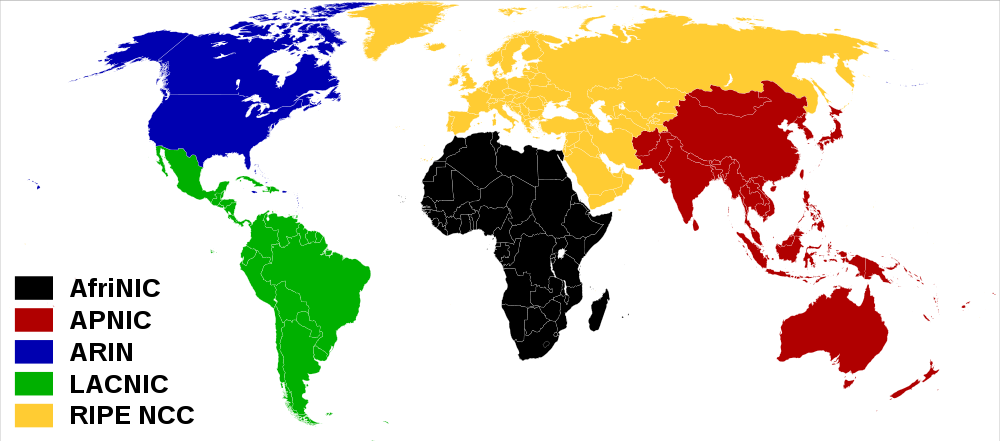
\includegraphics[scale=0.5]{pics/rirs.eps} \\
% 	\vspace{.5in}
% 	Regional Internet Registries (RIR) manage the allocation and
% registration of Internet number resources within a region of the world.
% \end{center}
% \vspace*{\fill}
%
% \subsection{Mommy, where do IP addresses come from?}
% \vspace*{\fill}
% \begin{center}
% {\bf RIR}s assign blocks of IP addresses to the Local Internet Registries (LIR).
% \\
% \vspace{.5in}
%
% LIRs are either ISPs, enterprises using a lot of addresses, or academic
% institutions.
% \end{center}
% \vspace*{\fill}
%
% \subsection{IPv4 Exhaustion}
% Past and predicted: \\
%
% \begin{tabular}{l r}
% IANA Address Pool Exhaustion: & 2011-02-03 \\
% APNIC reached final {\tt /8}: & 2011-04-15 \\
% RIPENCC: & 2012-09-14 \\
% LACNIC: & 2014-09-05 \\
% ARIN: & 2015-03-23 \\
% AFRINIC: & 2020-08-10 \\
% \end{tabular}
%
% \subsection{IPv6 Basics}
% \vspace{.5in}
% \Hugesize
% \begin{center}
% \begin{verbatim}
%        10011011111101100101100100010110
% \end{verbatim}
% \vspace{.5in}
% IPv4 addresses are 32-bit numbers.
% \end{center}
% \Normalsize
%
%
% \subsection{IPv6 Basics}
% \Hugesize
% \begin{center}
% \begin{verbatim}
%               0010000000000001
%               0000010011111000
%               0000000000000100
%               0000000000000111
%               0000001011100000
%               1000000111111111
%               1111111001010010
%               1001101001101011
% \end{verbatim}
% \vspace{.5in}
% IPv6 addresses are 128 bits.
% \end{center}
% \Normalsize
%
% \subsection{IPv6 Basics}
% \Hugesize
% \begin{center}
% IPv4: 32 bits $=>$ $2^{32}$ addresses \\
% \vspace{.5in}
% IPv6: 128 bits $=>$ $2^{128}$ addresses
% \end{center}
% \Normalsize
%
% \subsection{IPv6 Basics}
% \Hugesize
% \begin{center}
% IPv4: 32 bits $=>$ $4,294,967,296$ addresses \\
% \vspace{.5in}
% IPv6: 128 bits $=>$ $2^{128}$ addresses
% \end{center}
% \Normalsize
%
% \subsection{IPv6 Basics}
% \Hugesize
% \begin{center}
% IPv4: 32 bits $=>$ $4,294,967,296$ addresses \\
% \vspace{.5in}
% IPv6: 128 bits $=>$ $340,282,366,920,938,463,463,374,607,431,768,211,456$ addresses \\
% \vspace{.5in}
% \end{center}
% \Normalsize
%
% \subsection{IPv6 Basics}
%
% ``if the earth were made entirely out of 1 cubic millimetre grains of
% sand, then you could give a unique IPv6 address to each grain in 300
% million planets the size of the earth''
% \\
% \verb+http://www.potaroo.net/papers/isoc/2005-07/ipv6size.html+
% \\
%
% \verb|https://www.wolframalpha.com/input/?i=2^128+%2F+number+of+cells+in+human+body|
% \verb|https://www.wolframalpha.com/input/?i=2^128+%2F+number+of+atoms+in+human+body|
% \verb|%2F+number+of+people+on+earth|
%
% \subsection{IPv6 Basics}
% \begin{itemize}
% 	\item 8x16 bit fields (words) in case insensitive colon hexadecimal
% 		representation
% \begin{verbatim}
%            2031:0000:0000:130F:0000:0000:076A:130B
% \end{verbatim}
% \end{itemize}
%
% \subsection{IPv6 Basics}
% \begin{itemize}
% 	\item 8x16 bit fields (words) in case insensitive colon hexadecimal
% 		representation
% \begin{verbatim}
%            2031:0000:0000:130F:0000:0000:076A:130B
% \end{verbatim}
% 	\item Leading zeros in a field are optional:
% \begin{verbatim}
%            2031:0:0:130F:0:0:76A:130B
% \end{verbatim}
% \end{itemize}
%
% \subsection{IPv6 Basics}
% \begin{itemize}
% 	\item 8x16 bit fields (words) in case insensitive colon hexadecimal
% 		representation
% \begin{verbatim}
%            2031:0000:0000:130F:0000:0000:076A:130B
% \end{verbatim}
% 	\item Leading zeros in a field are optional:
% \begin{verbatim}
%            2031:0:0:130F:0:0:76A:130B
% \end{verbatim}
% 	\item Successive fields of 0 represented as ::, but only once in
% 			an address:
% \begin{verbatim}
%           2031::130F:0:0:76A:130B         ok
%           2031:0:0:130F::76A:130B         ok
%           2031::130F::76A:130B            not ok
% \end{verbatim}
% \end{itemize}
%
% \subsection{IPv6 Basics}
% \begin{itemize}
% 	\item 8x16 bit fields (words) in case insensitive colon hexadecimal
% 		representation
% \begin{verbatim}
%            2031:0000:0000:130F:0000:0000:076A:130B
% \end{verbatim}
% 	\item Leading zeros in a field are optional:
% \begin{verbatim}
%            2031:0:0:130F:0:0:76A:130B
% \end{verbatim}
% 	\item Successive fields of 0 represented as ::, but only once in
% 			an address:
% \begin{verbatim}
%           2031::130F:0:0:76A:130B         ok
%           2031:0:0:130F::76A:130B         ok
%           2031::130F::76A:130B            not ok
% \end{verbatim}
% 	\item
% \begin{verbatim}
%           0000:0000:0000:0000:0000:0000:0000:00001 =>
%                                    0:0:0:0:0:0:0:1 => ::1
% \end{verbatim}
% \end{itemize}
%
% \subsection{IPv6 Basics - Address Oddities}
% \begin{itemize}
% 	\item Address may include a link name:
% \begin{verbatim}
%           2001:470:1f07:3d1::1%eth0
% \end{verbatim}
% \end{itemize}
%
% \subsection{IPv6 Basics - Address Oddities}
% \begin{itemize}
% 	\item Address may include a link name:
% \begin{verbatim}
%           2001:470:1f07:3d1::1%eth0
% \end{verbatim}
% 	\item IPv4-mapped addresses
% \begin{verbatim}
%           0:0:0:0:0:ffff:66.163.162.9
%           ::ffff:66.163.162.9
% \end{verbatim}
% \end{itemize}
%
% \subsection{IPv6 Basics - Address Oddities}
% \begin{itemize}
% 	\item Address may include a link name:
% \begin{verbatim}
%           2001:470:1f07:3d1::1%eth0
% \end{verbatim}
% 	\item IPv4-mapped addresses
% \begin{verbatim}
%           0:0:0:0:0:ffff:66.163.162.9
%           ::ffff:66.163.162.9
% \end{verbatim}
% 	\item You need brackets to distinguish a port from an address:
% 		\begin{itemize}
% 			\item IPv4: \verb+66.163.162.9:22+
% 			\item IPv6: \verb+[2001:470:1f07:3d1::1]:22+
% 		\end{itemize}
% \end{itemize}
%
% \subsection{IPv6 Basics -- Address Scope}
% \begin{itemize}
% 	\item Link-Local (example: \verb+fe80::e276:63ff:fe72:3900%xennet0+)
% 		\begin{itemize}
% 			\item Used on a single link
% 			\item Packets with link-local source or destination addresses are not
% 				forwarded to other links
% 		\end{itemize}
% \end{itemize}
%
% \subsection{IPv6 Basics -- Address Scope}
% \begin{itemize}
% 	\item Link-Local (example: \verb+fe80::e276:63ff:fe72:3900%xennet0+)
% 		\begin{itemize}
% 			\item Used on a single link
% 			\item Packets with link-local source or destination addresses are not
% 				forwarded to other links
% 		\end{itemize}
% 	\item Unique-Local (\verb+fc00::/7+)
% 		\begin{itemize}
% 			\item Used for private IPv6 networks
% 			\item not globally routable
% 			\item Applications similar to RFC 1918
% 		\end{itemize}
% \end{itemize}
%
% \subsection{IPv6 Basics -- Address Scope}
% \begin{itemize}
% 	\item Link-Local (example: \verb+fe80::e276:63ff:fe72:3900%xennet0+)
% 		\begin{itemize}
% 			\item Used on a single link
% 			\item Packets with link-local source or destination addresses are not
% 				forwarded to other links
% 		\end{itemize}
% 	\item Unique-Local (\verb+fc00::/7+)
% 		\begin{itemize}
% 			\item Used for private IPv6 networks
% 			\item not globally routable
% 			\item Applications similar to RFC 1918
% 		\end{itemize}
% 	\item Global (example: \verb+2001:470:1f07:3d1::1+)
% 		\begin{itemize}
% 			\item A globally unique address
% 			\item Packets with global addresses can be forwarded to any part of
% 				the global network
% 		\end{itemize}
% \end{itemize}
%
% \subsection{IPv6 Configuration Types}
% \begin{itemize}
% 	\item Static Configuration
% 	\item Stateful Autoconfiguration (DHCPv6)
% 	\item Stateless Address Autoconfiguration (SLAC)
% \end{itemize}
%
% \subsection{IPv6 Configuration Types}
% \begin{itemize}
% 	\item Static Configuration
% 	\item Stateful Autoconfiguration (DHCPv6)
% 	\item Stateless Address Autoconfiguration (SLAC)
% 	\begin{itemize}
% 		\item RFC2462
% 		\item use of autonomously configured link-local address
% 			using its EUI-64 address
% \begin{verbatim}
%           fe80::213:d3ff:fe9c:1840%eth0
% \end{verbatim}
% 		\item at boot time, send Router Solicitation (RS) to
% 			request Router Advertisements (RAs)
% 	\end{itemize}
% \end{itemize}
%
% \subsection{IPv6 Subnets}
% \begin{verbatim}
% $ sipcalc 2001:470:30:84:e276:63ff:fe72:3900/64
% -[ipv6 : 2001:470:30:84:e276:63ff:fe72:3900/64] - 0
%
% [IPV6 INFO]
% Expanded Address        - 2001:0470:0030:0084:e276:63ff:fe72:3900
% Compressed address      - 2001:470:30:84:e276:63ff:fe72:3900
% Subnet prefix (masked)  - 2001:470:30:84:0:0:0:0/64
% Address ID (masked)     - 0:0:0:0:e276:63ff:fe72:3900/64
% Prefix address          - ffff:ffff:ffff:ffff:0:0:0:0
% Prefix length           - 64
% Address type            - Aggregatable Global Unicast Addresses
% Network range           - 2001:0470:0030:0084:0000:0000:0000:0000 -
%                           2001:0470:0030:0084:ffff:ffff:ffff:ffff
%
% \end{verbatim}
%
% \subsection{IPv6 Subnets: Common CIDRs}
% \small
% \begin{verbatim}
% 2001:0db8:0123:4567:89ab:cdef:1234:5678
% |||| |||| |||| |||| |||| |||| |||| |||128   Single end-points and loopback
% |||| |||| |||| |||| |||| |||| |||| ||124
% |||| |||| |||| |||| |||| |||| |||| |120
% |||| |||| |||| |||| |||| |||| |||| 116
% |||| |||| |||| |||| |||| |||| |||112
% |||| |||| |||| |||| |||| |||| ||108
% |||| |||| |||| |||| |||| |||| |104
% |||| |||| |||| |||| |||| |||| 100
% |||| |||| |||| |||| |||| |||96
% |||| |||| |||| |||| |||| ||92
% |||| |||| |||| |||| |||| |88
% |||| |||| |||| |||| |||| 84
% |||| |||| |||| |||| |||80
% |||| |||| |||| |||| ||76
% |||| |||| |||| |||| |72
% |||| |||| |||| |||| 68
% |||| |||| |||| |||64                        Single End-user LAN (default prefix size for SLAAC)
% |||| |||| |||| ||60
% |||| |||| |||| |56                          Proposed minimal end sites assignment
% |||| |||| |||| 52
% |||| |||| |||48                             Default end sites assignment
% |||| |||| ||44
% |||| |||| |40
% |||| |||| 36
% |||| |||32                                  Local Internet registry minimum allocations
% |||| ||28                                   Local Internet registry medium allocations
% |||| |24                                    Local Internet registry large allocations
% |||| 20                                     Local Internet registry extra large allocations
% |||16
% ||12                                        Regional Internet Registry allocations from IANA
% |8
% \end{verbatim}
% \Normalsize
%
% \subsection{How to know if you will be in trouble...}
% Go to \verb+http://test-ipv6.com+:
% \begin{center}
% 	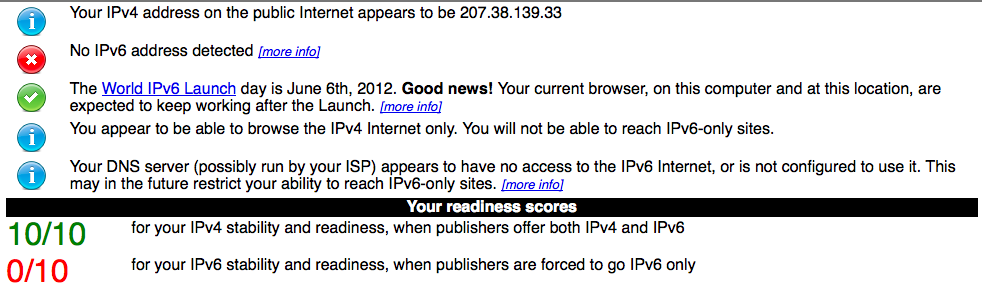
\includegraphics[scale=0.7]{pics/test-ipv6.eps}
% \end{center}
%
% \subsection{How to know if you will be in trouble...}
% Go to \verb+http://test-ipv6.com+:
% \begin{center}
% 	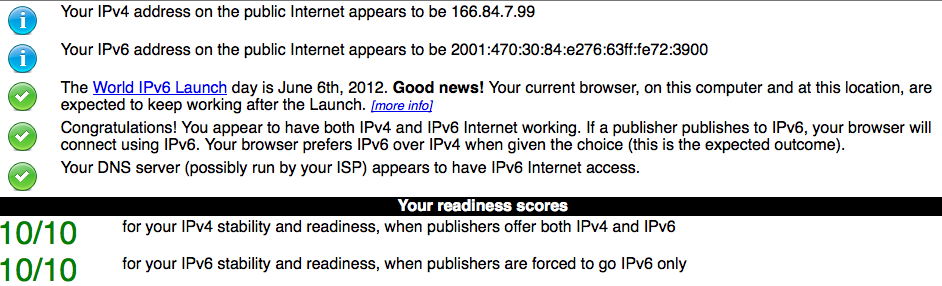
\includegraphics[scale=0.7]{pics/test-ipv6-6.eps}
% \vspace{.25in}
%
% If you don't have native IPv6 connectivity, use a tunnelbroker to connect
% IPv4-only hosts to the IPv6 internet. \\
%
% \verb+http://tunnelbroker.net/+
% \end{center}
%

\subsection{Internet Maps and Architecture}
\begin{itemize}
	\item \verb+http://www.peer1.com/map-of-the-internet+
	\item \verb+http://is.gd/VxsE7S+
	\item \verb+http://www.submarinecablemap.com/+
	\item \verb+http://en.wikipedia.org/wiki/Peering+
	\item \verb+http://is.gd/tpPNE5+
	\item \verb+http://is.gd/B0d3kh+
	\item \verb+http://amzn.com/0061994936+
\end{itemize}

\subsection{IPv6}
\begin{itemize}
	\item \verb+http://bgp.he.net/ipv6-progress-report.cgi+
	\item \verb+https://ipv6.he.net/statistics/+
	\item \verb+http://tunnelbroker.net/+
\end{itemize}

\subsection{Reading}
\begin{itemize}
	\item \verb+traceroute 216.81.59.173+ -- \verb+http://is.gd/qXVo2j+
	\item \verb+traceroute -m 254 -q1 obiwan.scrye.net+
\end{itemize}
\vspace{.5in}
Commands:
\begin{itemize}
	\item \verb+tcpdump(8)+
	\item \verb+ktrace(1)+ / \verb+strace(1)+
	\item \verb+tcp(4)+/\verb+ip(4)+
	\item \verb+netstat(1)+
\end{itemize}

\end{document}
